%
%   Prof. Dr. Julian Reichwald
%   auf Basis einer Vorlage von Prof. Dr. Jörg Baumgart
%   DHBW Mannheim
%
%
%	ACHTUNG: Für das Erstellen des Literaturverzeichnisses wird das modernere Paket biblatex
%			 in Kombination mit biber verwendet -- nicht mehr das ältere BibTex!
% 			 Bitte stellen Sie ggf. Ihre TeX-Umgebung
% 			 entsprechend ein (z.B. TeXStudio: Einstellungen --> Erzeugen --> Standard Bibliographieprogramm: biber)
%

\documentclass[
	12pt,
	BCOR=5mm,
	DIV=12,
	headinclude=on,
	footinclude=off,
	parskip=half,
	bibliography=totoc,
	listof=entryprefix,
	toc=listof,
	pointlessnumbers,
	plainfootsepline]{scrreprt}

%	Konfigurationsdatei einziehen
% !TEX root =  master.tex
% 		HYPERREF
%
\usepackage[
	hidelinks=true % keine roten Markierungen bei Links
]{hyperref}

% Zwei eigene Befehle zum Setzen von Autor und Titel. Ausserdem werden die PDF-Informationen richtig gesetzt.
\newcommand{\TitelDerArbeit}[1]{\def\DerTitelDerArbeit{#1}\hypersetup{pdftitle={#1}}}
\newcommand{\AutorDerArbeit}[1]{\def\DerAutorDerArbeit{#1}\hypersetup{pdfauthor={#1}}}
\newcommand{\Firma}[1]{\def\DerNameDerFirma{#1}}
\newcommand{\Kurs}[1]{\def\DieKursbezeichnung{#1}}
\newcommand*{\quelle}[1]{\par\raggedleft\footnotesize Quelle:~#1}


%		FONT AND INPUT ENCODING
%
\usepackage[T1]{fontenc}
\usepackage[utf8]{inputenc}

%		CALCULATIONS
%
\usepackage{calc} % Used for extra space below footsepline

%		LANGUAGE SETTINGS
%
\usepackage[ngerman]{babel} 	% German language
\usepackage[german=quotes]{csquotes} 	% correct quotes using \enquote{}

%\usepackage[english]{babel}   % For english language
%\usepackage{csquotes} 	% Richtiges Setzen der Anführungszeichen mit \enquote{}


%		BIBLIOGRAPHY SETTINGS
%
 \usepackage[backend=biber, autocite=footnote, style=authoryear, dashed=false]{biblatex} 	%Use Author-Year-Cites with footnotes
% \usepackage[backend=biber, autocite=inline, style=ieee]{biblatex} 	% Use IEEE-Style (e.g. [1])
% \usepackage[backend=biber, autocite=inline, style=alphabetic]{biblatex} 	% Use alphabetic style (e.g. [TGK12])

%%%% APA/Harvard-Style (bitte die nächten zwei Zeilen auskommentieren)
%\usepackage[backend=biber, style=apa]{biblatex} 	
%\DeclareLanguageMapping{german}{german-apa}

\DefineBibliographyStrings{ngerman}{  %Change u.a. to et al. (german only!)
	andothers = {{et\,al\adddot}},
}

%%% Uncomment the following lines to support hard URL breaks in bibliography 
%\apptocmd{\UrlBreaks}{\do\f\do\m}{}{}
%\setcounter{biburllcpenalty}{9000}% Kleinbuchstaben
%\setcounter{biburlucpenalty}{9000}% Großbuchstaben


\setlength{\bibparsep}{\parskip}		%add some space between biblatex entries in the bibliography
\addbibresource{bibliography.bib}	%Add file bibliography.bib as biblatex resource


%		FOOTNOTES 
%
% Count footnotes over chapters
\usepackage{chngcntr}
\counterwithout{footnote}{chapter}

%	ACRONYMS
%%%
%%% WICHTIG: Installieren Sie das neueste Acronyms-Paket!!!
%%%
\makeatletter
\usepackage[printonlyused]{acronym}
\@ifpackagelater{acronym}{2015/03/20}
  {%
    \renewcommand*{\aclabelfont}[1]{\textbf{\textsf{\acsfont{#1}}}}
  }%
  {%
  }%
\makeatother

%		LISTINGS
\usepackage{listings}	%Format Listings properly
\renewcommand{\lstlistingname}{Quelltext} 
\renewcommand{\lstlistlistingname}{Quelltextverzeichnis}
\lstset{numbers=left,
	numberstyle=\tiny,
	captionpos=b,
	basicstyle=\ttfamily\small}


%		EXTRA PACKAGES
\usepackage{lipsum}    %Blindtext
\usepackage{graphicx} % use various graphics formats
\usepackage[german]{varioref} 	% nicer references \vref
\usepackage{caption}	%better Captions
\usepackage{booktabs} %nicer Tabs
\usepackage{array}
%\newcolumntype{P}[1]{>{\raggedright\arraybackslash}p{#1}}


%		ALGORITHMS
\usepackage{algorithm}
\usepackage{algpseudocode}
\renewcommand{\listalgorithmname}{Algorithmenverzeichnis }
\floatname{algorithm}{Algorithmus}


%		FONT SELECTION: Entweder Latin Modern oder Times / Helvetica
\usepackage{lmodern} %Latin modern font
%\usepackage{mathptmx}  %Helvetica / Times New Roman fonts (2 lines)
%\usepackage[scaled=.92]{helvet} %Helvetica / Times New Roman fonts (2 lines)

%		PAGE HEADER / FOOTER
%	    Warning: There are some redefinitions throughout the master.tex-file!  DON'T CHANGE THESE REDEFINITIONS!
\RequirePackage[automark,headsepline,footsepline]{scrpage2}
\pagestyle{scrheadings}
\renewcommand*{\pnumfont}{\upshape\sffamily}
\renewcommand*{\headfont}{\upshape\sffamily}
\renewcommand*{\footfont}{\upshape\sffamily}
\renewcommand{\chaptermarkformat}{}

\clearscrheadfoot

\ifoot[\rule{0pt}{\ht\strutbox+\dp\strutbox}DHBW Mannheim]{\rule{0pt}{\ht\strutbox+\dp\strutbox}DHBW Mannheim}
\ofoot[\rule{0pt}{\ht\strutbox+\dp\strutbox}\pagemark]{\rule{0pt}{\ht\strutbox+\dp\strutbox}\pagemark}

\ohead{\headmark}


\begin{document}

%% BITTE GEBEN SIE HIER DEN TITEL UND DIE AUTORIN / DEN AUTOR DER ARBEIT AN!
%% DIESE INFORMATIONEN _MÜSSEN_ GESETZT SEIN, UM TITELBLATT, ABSTRACT UND 
%% EIGENSTÄNDIGKEITSERKLÄRUNG AUTOMATISCH ANZUPASSEN!
\TitelDerArbeit{Evaluation von Continuous Practices während des Entwicklungsprozesses und Bewertung von Alternativen im Hinblick auf den Betrieb im Clusterverbund}
\AutorDerArbeit{Paul Hermany}
\Firma{Atos Information Technology GmbH}
\Kurs{WWI16SEA}

\begin{titlepage}
\begin{minipage}{\textwidth}
		\vspace{-2cm}
		\noindent 
\includegraphics[scale=0.1]{img/Logo-Atos.jpg} \hfill   
\includegraphics{img/logo.jpg}
\end{minipage}
\vspace{1em}
\sffamily
\begin{center}
	\textsf{\large{}Duale Hochschule Baden-W\"urttemberg\\[1.5mm] Mannheim}\\[2em]
	\textsf{\textbf{\Large{}Bachelorarbeit}}\\[3mm]
	\textsf{\textbf{\DerTitelDerArbeit}} \\[1.5cm]
	\textsf{\textbf{\Large{}Studiengang Wirtschaftsinformatik}\\[3mm] \textsf{Studienrichtung Software Engineering}}
	
	\vspace{3em}
\vfill

\begin{minipage}{\textwidth}

\begin{tabbing}
	Wissenschaftlicher Betreuer: \hspace{0.85cm}\=\kill
	Verfasser: \> \DerAutorDerArbeit \\[1.5mm]
	Matrikelnummer: \> 2912279 \\[1.5mm]
	Firma: \> \DerNameDerFirma  \\[1.5mm]
	Abteilung: \> Softwareentwicklung \\[1.5mm]
	Kurs: \> \DieKursbezeichnung \\[1.5mm]
	Studiengangsleiter: \> Prof. Dr. Julian Reichwald  \\[1.5mm]
	Wissenschaftlicher Betreuer: \> Prof. Dr. Frank Hubert  \\
	\> frank.hubert@dhbw-mannheim.de \\
	\> +49 621 4105 1285 \\[1.5mm]
	Firmenbetreuer: \> Danny Tschorsch \\
	\> danny.tschorsch@atos.net \\
	\> +49 211 3993 2559 \\[1.5mm]
	Bearbeitungszeitraum: \> 26.11.2018 -- 18.02.2019
\end{tabbing}
\end{minipage}

\end{center}

\end{titlepage}

\pagenumbering{roman} % Römische Seitennummerierung
\normalfont

%--------------------------------
% Verzeichnisse - nicht benötige Verzeichnisse bitte auskommentieren / löschen.
%--------------------------------

%   Sperrvermerk
%\chapter*{Sperrvermerk}
Der Inhalt dieser Arbeit darf weder als Ganzes noch in Auszügen Personen außerhalb des Prüfungsprozesses und des Evaluationsverfahrens zugänglich gemacht werden, sofern keine anders lautende Genehmigung der Ausbildungsstätte vorliegt. 
\cleardoublepage


%	Kurzfassung
\chapter*{Kurzfassung}
\begingroup
\begin{table}[h!]
\setlength\tabcolsep{0pt}
\begin{tabular}{p{3.7cm}p{11.7cm}}
Titel & \DerTitelDerArbeit \\
Verfasser/in: & \DerAutorDerArbeit \\
Kurs: & \DieKursbezeichnung \\
Ausbildungsstätte: & \DerNameDerFirma\\
\end{tabular}
\end{table}
\endgroup

Hier können Sie die Kurzfassung der Arbeit schreiben.




%	Inhaltsverzeichnis
\tableofcontents

%	Abbildungsverzeichnis
\listoffigures

%	Tabellenverzeichnis
\listoftables

%	Listingsverzeichnis
 \lstlistoflistings

% 	Algorithmenverzeichnis
\listofalgorithms

% 	Abkürzungsverzeichnis (siehe Datei acronyms.tex!)
\clearpage
\chapter*{Abkürzungsverzeichnis}	
\addcontentsline{toc}{chapter}{Abkürzungsverzeichnis}


\begin{acronym}[RDBMS]
	\acro{AHP}{Analytic Hierarchy Process}
	\acro{CAP}{AITs-B\&PS-GER-TEC-AM CAP DB APP NordWest}
	\acro{CDE}{Continuous Delivery}
	\acro{CD}{Continuos Deployment}
    \acro{CI}{Continuous Integration}	
	\acro{CIx}{Consistency Index}
	\acro{CR}{Consistency Ratio}
	\acro{IaaS}{Infarstructure as a Service}
	\acro{NWA}{Nutzwertanalyse}	
    \acro{MCDA}{Multi Criteria Decision Analysis}	
	\acro{RI}{Random Consistency Index}
\end{acronym}


%--------------------------------
% Start des Textteils der Arbeit
%--------------------------------
\clearpage
\ihead{\chaptername~\thechapter} % Neue Header-Definition
\pagenumbering{arabic}  % Arabische Seitenzahlen

%	Anleitungs-Datei anleitung.tex einziehen. Auf diese Weise sollten Sie versuchen, für jedes einzelne
% Kapitel eine eigene Datei anzulegen und mittels input-Kommando einzuziehen.
% !TEX root =  master.tex
%\section{Zieldefinition}
%Das Ziel dieser Arbeit ist es zum einen die Vorteile von Continuous Integration und Continuous Deployment aufzuzeigen und zum anderen verschiedenen Systeme für CI \& CD untereinander zu vergleichen. Das Aufzeigen der Vorteile wird dabei als Aufhänger genutzt um in das Thema einzuleiten. Der Praxisbezug wird durch das Problem der Abteilung hergestellt. Deren CI/CD Pipeline braucht mittlerweile mehr als 20 Minuten um einen Durchlauf abzuschließen. Aus diesem Grund haben Sie sich dazu entschlossen die Pipeline auf einen Cluster aufzuteilen, dabei übernehmen die einzelnen Knoten im Cluster spezialisierte Aufgaben. Ein Knoten kümmert sich zum Beispiel um die Unit-Tests und ein weiterer um Komponententests durchzuführen. Dadurch soll die Zeit für eine Durchlauf reduziert werden. Um diese Cluster aufzubauen gibt es viele Möglichkeiten von vielen Anbietern. Sowohl in der Cloud als auch On Premise. Da die Ressourcen der Abteilung beschränkt sind wollen sie natürlich die am Besten zu ihnen passende Lösung. Mit dieser Problemstellung wird sich diese Arbeit größtenteils beschäftigen. Am Ende der Arbeit soll eine Handlungsempfehlung für die Abteilung vorliegen an der sie sich orientieren kann.
%\section{Untersuchungsmethodik}
%Damit die Alternativen möglichst objektiv bewertet werden können soll eine AHP-Analyse(Analytic Hierarchy Process) durchgeführt werden. Dabei ist das Ziel möglichst viele Stakeholder an der Aufstellung des Kriterienkatalogs und der Gewichtung teilhaben zu lassen.
\chapter{Einleitung} 
\section{Motivation} 
\section{Problemstellung} 
\section{Zielsetzung} 
\chapter{Theoretische Grundlagen} 
Im folgenden Abschnitt werden die theoretischen Grundlagen geschaffen, die für das Verständnis dieser Arbeit relevant sind. Auf der technischen Seite werden sowohl Continuous Integration und Continuous Deployment als auch Versionsverwaltungssysteme erläutert. Ein Überblick über die Methodik der Arbeit wird mit der AHP-Analyse gegeben.
\section{Analytic Hierarchy Process (AHP-Analyse)}
Wie kann man rationale Entscheidungen in einer irrationalen Welt treffen? Man kann es nicht. Allerdings ist es möglich mithilfe von verschiedenen Analysemethoden der Entscheidungstheorie eine möglichst große Näherung an eine rationale Entscheidung zu erreichen. 
\subsection{Einführung}
Eine dieser Methoden ist die \ac{NWA}. Sie ist ein bewährtes Hilfsmittel in Wissenschaft und Wirtschaft, um Entscheidungen zu finden und Möglichkeiten zu bewerten. Indem das Problem fragmentiert wird, kann durch die Methodik der Nutzwertanalyse die vollständige Problematik erfasst werden, oder anders ausgedrückt: \enquote{Das Gesamtproblem, das es zu entscheiden gilt, wird in Teilprobleme zerlegt und diese, wenn erforderlich, wiederum in Teilprobleme}\autocite[S.1]{Kuehnapfel.2014}. Alle Facetten des Problems werden betrachtet und nicht vereinfacht oder abstrahiert. Somit umgeht man die menschliche Natur, die aufgrund einer möglichen Zeitersparnis ein komplexes Problem immer vereinfachen will. Das Vereinfachen führt allerdings zu einer erhöhten Fehlerquote und zum sofortigen Ausschluss von unkonventionellen Möglichkeiten aufgrund der Tendenz des Menschen zu Konstanz und Bewahrung\autocite[Vgl.][S.1]{Kuehnapfel.2014}. Im Gegensatz dazu gewährleistet die Nutzwertanalyse Objektivität und Chancengleichheit unter den verschiedenen Alternativen.\newline
Die Rationalität der Methodik ergibt sich aus der Vorgehensweise bei der Bearbeitung einer Fragestellung. Die einzelnen Fragmente (Kriterien) der Fragestellung werden einzeln bewertet und entsprechend ihrer Relevanz am Gesamtproblem gewichtet.\autocite[Vgl.][S.10]{Kuehnapfel.2014} An der Auswahl der Kriterien und deren Gewichtung sollten möglichst viele Stackeholder beteiligt sein um die Einflussnahme einzelner Meinungen zu unterbinden.\\
\\
In den 1970er Jahren hat Thomas L. Saaty das Konzept der \ac{NWA} weiterentwickelt. Der \ac{AHP} ist wie die \ac{NWA} ein grundlegender Ansatz zur Entscheidungsfindung und wurde entworfen um sowohl rationale als auch intuitive Entscheidungen in die Auswahl von zuvor selektierten Alternativen einzubeziehen.\autocite[Vgl.][S.1]{Saaty.2012} Er heißt Analytischer Hierarchie Prozess weil er sowohl analytisch, hierarchisch als auch prozessorientiert arbeitet.\autocite{TUM.2015}
\begin{itemize}
	\item\texttt{analytisch:} Die Entscheidungsunterstützung erfolgt mathematisch und mittels Logik
	\item\texttt{hierarchisch:} \enquote{Bei Nutzung des AHP sind die für die Erfüllung der Zielstellung genutzten Entscheidungskriterien einer hierarchischen Struktur unterworfen.}\autocite[S.314]{Hausladen.2016} 
	\item\texttt{prozessorientiert:} Die Entscheidungsunterstützung erfolgt immer nach dem selben Prozess
\end{itemize}
Während des Prozesses werde einfache paarweise Vergleiche durchgeführt. Die Ergebnisse dieser Vergleiche werden dann genutzt um eine Reihenfolge der Alternativen zu erstellen.\autocite[Vgl.][S.1]{Saaty.2012}
\subsection{Ablauf des AHP}
Die einfachste Form ein Entscheidungsproblem in einer AHP-Analyse darzustellen ist innerhalb einer Hierarchie mit drei Ebenen.(Abbildung \ref{img:hier})
\begin{figure}[h!]
	\centering
	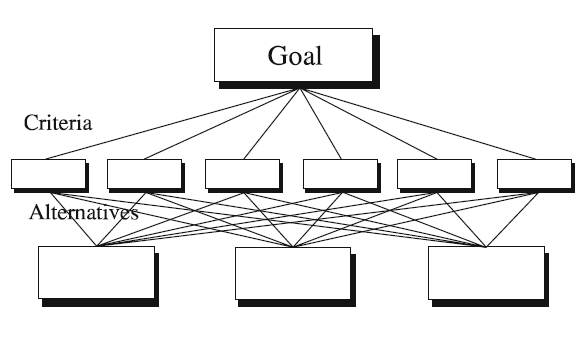
\includegraphics[scale = 0.8]{img/Hierarchie.png}
	\quelle{\cite[S.3]{Saaty.2012}}
	\caption{three level hierarchie}
	\label{img:hier}
\end{figure}
Das Grundproblem wird immer weiter granuliert. Auf der untersten Ebene finden sich die Alternativen welche mithilfe der Kriterien auf Ebene 2 evaluiert werden. Diese Erkenntnisse werden dann genutzt um das Ziel der Entscheidung auf der obersten Ebene zu bestimmen.\autocite[Vgl.][S.2]{Saaty.2012}
Damit hat man auch gleich den Startpunkt einer AHP-Analyse bestimmt. 
\subsubsection{Aufstellen des Entscheidungsmodells}
Die Analyse beginnt, wie oben bereits beschrieben mit dem Aufstellen des hierarchischen Entscheidungsmodells. Aus dem Entscheidungsproblem wird ein Ziel definiert, welchem eine endliche Anzahl von Alternativen zugeordnet wird $X=\{x_{1}, ..., x_{n}\}$\autocite[Vgl.][S.3]{Brunelli.2015}.
Des Weiteren werden die Kriterien für ... aus dem Ziel abgeleitet. Sollte die Kriterienanzahl zu groß sein bietet es sich an diese in Subkriterien aufzuteilen. Dadurch erhält man eine weitere Ebene innerhalb der Hierarchie. Am Ende dieser Phase der AHP-Analyse sollte eine Struktur ähnlich zu Abbildung \ref{img:hier} vorhanden sein. Mit dieser fertig erstellten Hierarchie erhält man eine bessere Übersicht über die Entscheidung die gefällt wird, die Kriterien die genutzt werden und die Alternativen die zur Verfügung stehen.\autocite[Vgl.][S.9]{Mu.2018} 
\subsubsection{Gewichtung der Kriterien}
Nicht alle Kriterien werden die gleiche Relevanz haben. Deswegen werden im zweiten Schritt der AHP-Analyse die Kriterien gewichtet.\autocite[Vgl.][S.9]{Mu.2018} Und zwar relativ zueinander. Relativ bezieht sich dabei auf den Umstand, dass für die Priorisierung der einzelnen Kriterien, diese im Verhältnis zueinander bestimmt werden. \\
Damit die Gewichtungen vergleichbar sind, besonders wenn diese in einem Bewertungsgremium getroffen werden, muss es eine zentrale Skala geben. Mithilfe dieser werden dann die entsprechenden Gewichtungen vorgenommen. Am Ende diese Prozesses soll ein Gewichtungsvektor $w=(w_{1}, ..., w_{n})$ mit einem $w_i$ für jedes $x_i$ aus $X=\{x_{1}, ..., x_{n}\}$ entstehen\autocite[Vgl.][S.4]{Brunelli.2015}. \\
\begin{figure}[h!]
	\centering
	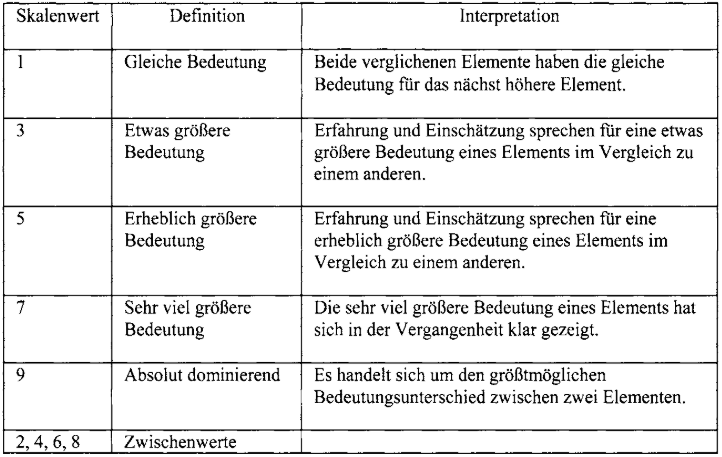
\includegraphics[scale = 0.8]{img/Skala.png}
	\quelle{\cite[S.105]{Fink.2006}}
	\caption{Saaty-Skala}
	\label{img:scale}
\end{figure}
Die Schwierigkeit dabei ist die Auswahl der richtigen/passenden Skala. In seinem 1977 veröffentlichen Artikel\autocite{Saaty.1977} vergleicht Saaty verschiedene Skalen miteinander und kommt dabei zu dem Entschluss, dass die Skala von 1-9 (Abbildung \ref{img:scale}) die passendste, im Hinblick auf die Anwendung mit der AHP-Analyse, ist. \\
Mithilfe dieser Skala werden nun die paarweise Vergleiche durchgeführt. Jede Kategorie wird mit jeder anderen einzeln verglichen und mithilfe der Skala bewertet.\autocite[Vgl.][S.106]{Fink.2006}  
\[\begin{array}{rcl}
		\centering
	  x_1 &\leftrightarrow &x_2 \\
	  x_1 &\leftrightarrow &x_3 \\
	  x_2 &\leftrightarrow &x_3 \\
   \vdots &                &\vdots
\end{array}\]
Am Ende dieses Prozesses sollte eine Matrix ähnlich zu \ref{matrix} entstanden sein.
\begin{table}[h!]
    \centering
\[X\quad = \quad\begin{tabular}{l|llll}
		& $x_1$ & $x_2$ &  $x_3$  \\ \hline
  $x_1$ &   1   &   5   &   2   \\
  $x_2$	&$\frac{1}{5}$&   1   &$\frac{1}{3}$     \\
  $x_3$	&$\frac{1}{2}$&   3   &   1         
   	  \end{tabular} 	  
\quad bzw. \quad
\left( \begin{array}{rrrr}
 1   &   5   &   2   \\
\frac{1}{5}&   1   &\frac{1}{3}     \\
\frac{1}{2}&   3   &   1        
\end{array}\right) 
\]
\caption{Matrix}
\label{matrix}
\end{table}
In diesem Beispiel lässt sich erkennen, dass $x_1$ erheblich größere Bedeutung hat als $x_2$. Außerdem hat $x_3$ etwas größere Bedeutung als $x_2$.
\subsubsection{Gewichtungsvektoren}
Mit dieser Tabelle lassen sich jetzt aber noch keine Aussagen treffen. Deswegen werden in diesem Arbeitsschritt die Gewichtungsvektoren $w=(w_{1}, ..., w_{n})$ berechnet.\\
Hierfür gibt es zwei Methoden. Das Näherungsverfahren und die Eigenvektormethode. Die Eigenvektormethode kann dabei als theoretischer Grundbaustein der AHP-Analyse angesehen werden.\autocite[Vgl.][S.106]{Fink.2006} Für die nachfolgende Erklärung wird allerdings das Näherungsverfahren beschrieben. Dieses führt\enquote{im Falle vollkommen konsistenter Urteile ebenfalls zu exakten Ergebnissen}\autocite[S.106]{Fink.2006}.
\begin{figure}[h!]
	\centering
	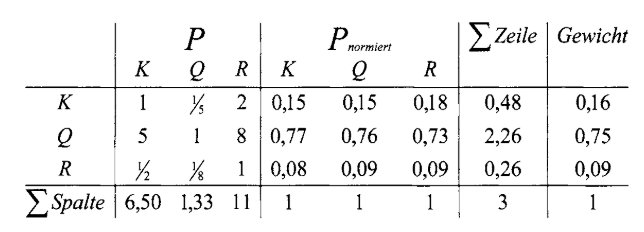
\includegraphics[scale = 0.9]{img/Tabelle.png}
	\quelle{\cite[S.107]{Fink.2006}}
	\caption{Paarvergleichsmatrix}
	\label{img:table}
\end{figure}
Die Berechnung beginnt mit der Normalisierung der Matrix aus dem vorangegangenen Arbeitsschritt. Dafür werden die Spalten zuerst aufsummiert. Danach teilt man jede einzelne Zelle durch die Summe ihrer Spalte. Sobald dies erledigt ist erhält man das $P_{normiert}$ aus Abbildung \ref{img:table}. Für die abschließenden Gewichtungen müssen jetzt nur noch die Summen der Spalten gebildet werden und durch die Anzahl der Kriterien $n$ geteilt werden. In dem Beispiel \ref{img:table} ergibt sich daraus folgende Reihenfolge für die Kriterien: $Q > K > R$. \\
Hierbei handelt es sich um sogenannten lokale Prioritäten. Saaty teilt die errechneten Prioritäten in lokal und global ein.\autocite[Vgl.][S.16]{Saaty.2012} Dies bezieht sich auf die Gültigkeit der Gewichtungen innerhalb der Hierarchie. Lokale Prioritäten sind nur in ihrer Ebene gültig. Globale Prioritäten gelten für die gesamte Hierarchie. Aus den lokalen Prioritäten lassen sich aber einfach Globale berechnen. Sie werden einfach mit den nächsthöheren Ebenen multipliziert $w_n * w_{n-1}$\autocite[Vgl.][S.107]{Fink.2006}. 
\subsubsection{Konsistenz}
Wenn die Gewichtungen getroffen sind müssen sie auf ihre Konsistenz geprüft werden.\autocite[Vgl.][S.13]{Mu.2018} Sowohl ordinale Transitivität als auch kardinale Konsistenz müssen im Rahmen dessen liegen was Saaty beschrieben hat.\autocite[Vgl.][S.107]{Fink.2006} Die ordinale Transitivität ergibt sich aus der reinen Logik. Wenn $A > B$ und $B > C$ dann muss auch $A > C$ gelten.\autocite[Vgl.][S.108]{Fink.2006} Die kardinale Konsistenz gibt des weiteren an ob die Gewichtungen konsistent sind. \enquote{Ist A zwei Mai besser als B und B drei Mai besser als C, so ist kardinale Konsistenz nur dann gegeben, wenn A sechs Mai besser als C ist.}\autocite[S.107]{Fink.2006} Wenn allerdings Zwischenwerte wie 4, 5 oder 7 zugewiesen werden, kann es zu Inkonsistenzen kommen. In bestimmten Maßen ist dies erlaubt. Sie dürfen nur eine Grenze nicht überschreiten.\autocite[Vgl.][S.13]{Mu.2018} Diese ist mit $CR<=0.10$ festgesetzt. CR bedeutet \enquote{Consistency Ratio} und setzt sich wie folgt zusammen:\autocite[Vgl.][S.13]{Mu.2018}\\
\[CR=\frac{\mbox{\ac{CI}}}{\mbox{\ac{RI}}}\]\\
\ac{CI} beschreibt den Consistency Index der zuvor erstellten Matrix. Dieser errechnet sich indem man die Spalten der Ausgangsmatrix \ref{matrix} mit den errechneten Gewichtungen aus \ref{img:table} multipliziert (Siehe Abbildung \ref{img:crit}).
\begin{figure}[h!]
	\centering
	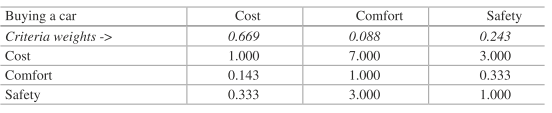
\includegraphics[scale = 1]{img/Kriterien.png}
	\quelle{\cite[S.12]{Mu.2018}}
	\caption{Prioritäten als Faktoren}
	\label{img:crit}
\end{figure}
Danach werden wieder die Summen der Spalten gebildet und durch die jeweiligen Gewichtungen geteilt. Die Ergebnisse werden aufsummiert und durch die Anzahl der Kriterien $n$ geteilt um den Durchschnitt zu errechnen (Siehe Abbildung \ref{img:lambda}). \\
\begin{figure}[h!]
	\centering
	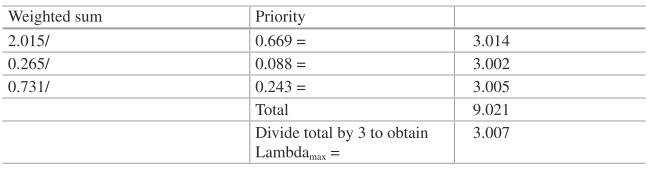
\includegraphics[scale = 0.9]{img/Lambda.png}
	\quelle{\cite[S.14]{Mu.2018}}
	\caption{Berechnung von $\lambda_{max}$}
	\label{img:lambda}
\end{figure} 
Mit $\lambda_{max}$ lässt sich nun der \ac{CI} von unserer Matrix berechnen. \\
Denn der \ac{CI} lässt sich wie folgt berechnen:\autocite[Vgl.][S.14]{Mu.2018}
\[CI=\frac{(\lambda_{max}-n)}{(n-1)}\quad \mbox{bzw. für unser Beispiel}\quad CI=\frac{(3.007-3)}{(3-1)}=0.004\]
Damit wir jetzt die \ac{CR} berechnen können fehlt uns nur noch der \ac{RI}. Hierbei handelt es sich um den \ac{CI} einer zufällig gefüllte Matrix welche der Theorie nach sehr inkonsistent sein muss. Saaty stellt praktischerweise schon den durchschnittlichen \ac{CI} von 500 zufällig gefüllten Matrizen zur Verfügung (Siehe Abbildung \ref{img:ri}).\\
\begin{figure}[h!]
	\centering
	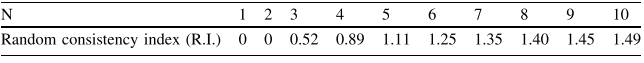
\includegraphics[scale = 0.9]{img/RI.png}
	\quelle{\cite[S.9]{Saaty.2012}}
	\caption{Durchschnittlicher RI}
	\label{img:ri}
\end{figure}\\
Diese sind nach $n$ geordnet und müssen jetzt nur noch in unsere Formel $CR=\frac{\mbox{\ac{CI}}}{\mbox{\ac{RI}}}$ eingesetzt werden.
\[CR=\frac{\mbox{\ac{CI}}}{\mbox{\ac{RI}}}=\frac{0.004}{0.52}=0.008\]
Es zeigt sich das $0.008<0.10$. Somit ist die kardinale Konsistenz gegeben und es kann fortgefahren werden. Sollte dies nicht gegeben sein muss die Matrix noch einmal überarbeitet werden um die inkonsistente Stellen zu eliminieren.\autocite[Vgl.][S.108]{Fink.2006}
\subsubsection{Gewichtung der Alternativen}
Nach der Gewichtung der Kriterien werden in diesem Arbeitsschritt die Gewichtungen für die Alternativen berechnet. Die Alternativen werden, wie die Kriterien vorher, paarweise verglichen. Allerdings immer im Hinblick auf ein Kriterium. Hat man also zum Beispiel 3 Kriterien, werden die Alternativen 3 mal im Hinblick auf die Kriterien verglichen. Am Ende entstehen dann 3 Matrizen. 
\begin{figure}[h!]
	\centering
	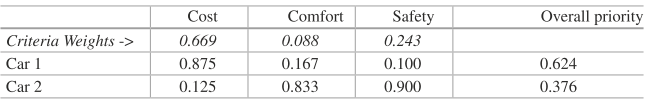
\includegraphics[scale = 0.9]{img/All.png}
	\quelle{\cite[S.19]{Mu.2018}}
	\caption{Modellsynthese}
	\label{img:all}
\end{figure}
Diese werden zusammengefasst und die einzelnen Spalten mit den jeweiligen Prioritäten der Kriterien multipliziert\autocite[Vgl.][S.19]{Mu.2018} (Siehe Abbildung \ref{img:all}) Abschließend werden die Summen der Zeilen gebildet. Die Ergebnisse sind dann die globalen Prioritäten und geben die abschließende Reihenfolge der Alternativen an. 
\subsubsection{Sensitivitätsanalyse}
Diese abschließenden Prioritäten sind sehr stark von der Gewichtung der Kriterien beeinflusst.\autocite[Vgl.][S.19]{Mu.2018} Aufgrund dessen wird als letzter Schritt, vor der abschließenden Bewertung, noch eine Sensitivitätsanalyse durchgeführt. Mithilfe dieser wird geprüft wie \enquote{robust} das Ergebnis der Analyse ist.\autocite[Vgl.][S.20]{Mu.2018} \enquote{Ziel ist es, durch die systematische Verlagerung von Kriteriengewichten Grenzen zu bestimmen, bei denen sich die Reihung von Altemativen umkehrt.}\autocite[S.111]{Fink.2006}\\ 
Getestet wird dies indem der letzte Schritt der Analyse noch einmal mit veränderten Gewichtungen vorgenommen wird. Was passiert also bei (a) gleichen Gewichtungen und (b) welche Gewichtung führen zu gleichen Prioritäten.\autocite[Vgl.][S.20]{Mu.2018}\\
Zuerst werden die Gewichtungen aller Kriterien gleichgesetzt. Bei 3 Kategorien würde dies eine jeweilige Gewichtung von $0.333$ bedeuten.\\
Um den \enquote{Break-Even Punkt}\autocite[S.21]{Mu.2018} der Prioritäten zu berechnen kann man sich mithilfe des Ergebnisses aus (a) herantasten. Durch das wiederholte umstellen der Prioritäten ist es möglich den \enquote{Break-Even Punkt} zu berechnen. Abschließend werden die Ergebnisse analysiert. \enquote{Führen bereits geringfügige Veränderungen der Kriteriengewichte zu einer [Umkehr der Prioritäten], so ist das ein Hinweis auf ein instabiles Ergebnis. In einem solchen Fall ist es ratsam, den Beurteilungsprozess zu wiederholen bzw. zu überprüfen.}\autocite[S.111]{Fink.2006}
\subsubsection{Finale Entscheidung}
Nachdem alle Schritte vollzogen sind kann eine finale Entscheidung gefällt werden. Dafür werden die Ergebnisse der Analyse, der Konsistenzanalyse und der Sensitivitätsanalyse einbezogen um eine aussagekräftige Entscheidung zu treffen, welche Alternative das festgelegte Ziel in Schritt 1 am besten erfüllt.
\subsection{Vergleich mit NWA}
fdfgfftzdf
\section{Versionsverwaltungssysteme}
In der heutigen Softwareentwicklung besteht ein Projekt aus vielen Quellcode-Dateien, die ständig neu erstellt und verändert werden. Um jegliche Veränderungen an dem Quellcode zu dokumentieren und nachvollziehen zu können, wird ein Versionskontrollsystem (Version Control System; VCS) genutzt.\autocite[Vgl.][S.6]{Baerisch.2005}  
Dieses ermöglicht es dem Entwickler beispielsweise, Weiterentwicklungen durchzuführen, während parallel an der aktuellen Version Fehler behoben werden. Darüber hinaus erlaubt eine Versionsverwaltung dem Entwickler, Änderungen mit anderen zu teilen und Änderungen von verschiedenen Personen zusammenzuführen.\autocite[Vgl.][S.9]{Kleine.2012} \\
Ein VCS bietet die Möglichkeit, Änderungen von Informationen beispielsweise an einem Quellcode zu organisieren und zu verwalten. \autocite[Vgl.][S.1]{Pilato.2009}
Die wachsende Sammlung an Informationen dient als „Repository (Lager), Projektgeschichte, Kommunikationsmedium und Werkzeug zur Team- und Produktverwaltung“.\autocite[][S.1]{Loeliger.2010} In einer Versionsverwaltung lagern somit nicht nur die Quelldateien, sie dient auch als Kernstück für ein ganzes Entwicklungsprojekt. \\
Zentrale Aufgaben der Versionsverwaltung sind der Zugriff auf historische Versionen der Dateien, Aufzeichnung der Änderungen in einem Log und die Entwicklung und Pflege eines Repository mit Inhalten. Die Aufbewahrung von älteren Versionen ist gerade in der Softwareentwicklung wichtig, da Software nach dem „Probierprinzip“\autocite[][S.9]{Versteegen.2003} entwickelt wird. Auf eine neue Entwicklung folgt ein anschließender Test. Es werden so lange Anpassungen durchgeführt und getestet, bis das optimale Ergebnis erreicht wurde.\autocite[Vgl.][S.9]{Versteegen.2003}
Ein Tool zur Sourcecodeverwaltung ermöglicht zudem das Management von Änderungen und den Zugriff von mehreren Entwicklern am gleichen Projekt.\autocite[Vgl.][S.1]{Loeliger.2010} Dies fördert die kollaborative Zusammenarbeit an einem Projekt, da parallel unterschiedliche Entwicklungen von mehreren Personen getätigt werden können. Gerade bei der Arbeit in einem Team muss die Möglichkeit der parallelen Entwicklung gegeben sein, da sich sonst die Entwickler in ihrer Arbeit gegenseitig beeinträchtigen.
\section{Continuous Integration, Continuous Delivery und Continuous Deployment}
Wie bewältigt man die größer werdende Nachfrage von Unternehmen und dem eigenen Management nach kürzeren Time-to-Market(Also der Zeit von der Entwicklung bis zum fertigen Produkt) und einer erhöhten Flexibilität und Agilität bei der Entwicklung?\autocite{Capgemini.2017} Continuous Integration, Continuous Delivery und Continuous Deployment (Auch Continuous Practices genannt) sind Techniken um genau diesen Prozess zu unterstützen.  Sie bieten die Möglichkeit die Geschwindigkeit des Entwicklungsprozesses zu erhöhen ohne Qualität einzubüßen.\autocite[Vgl.][S.2]{Shahin.2017}
Die Idee hinter Continuous Integration ist dabei nicht sonderlich neu. Bereits in den 90er Jahren wurde die Idee im größeren Kontext von Extreme Programming und dem Agilen Manifest erwähnt.\autocite[Vgl.][S.2]{Stahl.2018} Auch die grundlegende Idee, eine große Aufgabe in viele kleine Teile zu zerlegen und diese dann einzeln zu bearbeiten, ist nicht neu.\\ Über die Jahre hat sich die Idee weiterentwickelt und wurde von immer mehr Entwicklerteams aufgegriffen. Später kamen dann noch Continuous Delivery und Continuous Deployment hinzu die mithilfe von Automatisierung den Prozess weiter ausbauten und beschleunigten. Die Abgrenzung zwischen den Begriffen ist dabei nicht genau definiert, weswegen für viele zum Beispiel Teile der Continuous Delivery noch zu Continuous Integration gehören und für andere wiederum nicht. Insgesamt sollen aber alle Continuous Practices zu positiven Veränderungen führen.\autocite[Vgl.][S.2]{Shahin.2017}
\begin{itemize}
	\item Häufigeres und schnelleres Feedback aus dem Entwicklungsprozess und vom Kunden selbst 
	\item Erhöhte Releasezyklen mit stabilen Produkten führt zu erhöhter Produktqualität und verbesserter Kundenzufriedenheit
	\item Manuelle Aufgaben werden automatisiert
\end{itemize}
Im Folgenden wird nun auf die drei Hauptpractices im Detail eingegangen: Continuous Integration, Continuous Delivery und Continuous Deployment. Es existieren noch einige weitere Begriffe, allerdings sind die drei am bekanntesten und sind dem entsprechend am häufigsten im Einsatz. Es wird beschrieben was sie sind und was sie nicht sind. 
\subsection{Continuous Integration}
Continuous Integration ist wohl die bekannteste aller Practices und wird immer wieder als Synonym für alle Continuous Practices genannt.\autocite[Vgl.][S.12]{Stahl.2018} Dabei ist es per Definition nur \enquote{eine Softwarenetwicklungspraktik, bei der Entwickler, aus einem Team, ihre Veränderungen häufig in das Projekt integrieren. Mindestens einmal täglich}\autocite[S.12]{Stahl.2018}\\
Dies ist wichtig wenn die Größe des Entwicklungsteams über 1 wächst. Denn sobald mehrere Leute an einem Projekt arbeiten wird es schwieriger die Veränderungen des einen Entwicklers mit denen des anderen zu verknüpfen und das Programm zum laufen zu kriegen.\autocite[Vgl.][S.4]{Stahl.2018}\\ Mann kann es sich so vorstellen als wenn viele Autoren zusammen an einem sehr langen Roman arbeiten. Die Geschichte und alle Charaktere müssen konsequent geschrieben sein damit das Buch funktioniert. Je mehr Autoren mitarbeiten umso schwieriger wird es die einzelnen Teile zusammenzuführen.\\ Das gleiche Problem tritt auch in der Softwareentwicklung auf und wird komplizierter mit jedem Entwickler der dazu kommt. Außerdem wird es umso schwieriger wenn Veränderungen von einem Entwickler länger zurückgehalten werden. Je umfangreicher die Veränderungen sind die eingebracht werden umso schwieriger wird es diese zu integrieren. Dies bringt uns wieder zur Definition vom Anfang. Es geht nicht darum so oft und schnell wie möglich zu integrieren, sondern um die Häufigkeit und Regelmäßigkeit.\autocite[Vgl.][S.3]{Stahl.2018} Es beschleunigt den gesamten Entwicklungsprozess, da weniger Ressourcen für das Integrieren gebraucht werden. Des weiteren bildet Continuous Integration die Grundlage für Continuous Delivery und Continuous Deployment. Ohne kontinuierliches Integrieren bringen diese beiden Practices keinen Vorteil.
\subsection{Continuous Delivery}
2010 haben Jez Humble und David Farley
\subsection{Continuous Deployment}
\subsection{DevOps}
\subsection{Testdriven Programming}  
\chapter{Praktische Umsetzung}
\section{Projektumfeld}
\section{IST-Zustand}
\section{Zieldefinition}
\section{Kriterienkatalog}
\section{Auswahl der Zieltechnologien}
\section{Analyse}
\subsection{Aufstellung des Zielsystems}
\subsection{Gewichtung der Kriterien}
\subsection{Gewichtung der Alternativen}
\subsection{Berechnung der Gesamtgewichtung}
\subsection{Bewertung der Alternativen}
\section{Handlungsempfehlung}
\chapter{Zusammenfassung}
\section{Fazit} 
\section{Kritische Reflexion}


%	Literaturverzeichnis
\ihead{} % Neue Header-Definition
\printbibliography[title=Literaturverzeichnis]
\cleardoublepage

% Der Anhang beginnt hier - jedes Kapitel wird alphabetisch aufgezählt. (Anhang A, B usw.)
\appendix
\ihead{\appendixname~\thechapter} % Neue Header-Definition

% appendix.tex einziehen
%\chapter{Testanhang}
\lipsum



\section{Subtestanhang}

\chapter{Noch ein Testanhang}



% Ehrenwörtliche Erklärung ewerkl.tex einziehen
% !TEX root =  master.tex

\clearpage
\chapter*{Ehrenwörtliche Erklärung}

% Wird die folgende Zeile auskommentiert, erscheint die ehrenwörtliche
% Erklärung im Inhaltsverzeichnis.

% \addcontentsline{toc}{chapter}{Ehrenwörtliche Erklärung}
Ich versichere hiermit, dass ich die vorliegende Arbeit
 mit dem Thema: \textit{\DerTitelDerArbeit} selbstständig verfasst und keine anderen als die angegebenen Quellen und
Hilfsmittel benutzt habe. Ich versichere zudem,
dass die eingereichte elektronische Fassung mit der gedruckten Fassung übereinstimmt.

\vspace{3cm}
Ort, Datum \hfill \DerAutorDerArbeit



\end{document}
